\documentclass[a4paper,11pt]{book}
\usepackage{a4wide}
\usepackage{graphicx}
\usepackage{hyperref}
\usepackage{multirow}
\usepackage{underscore}

\newenvironment{myindentpar}[1]%
	{\begin{list}{}%
			{\setlength{\leftmargin}{#1}}%
			\item[]%
	}
{\end{list}}
	
\begin{document}

\begin{titlepage}
\begin{center}
% Upper part of the page. The '~' is needed because \\
% only works if a paragraph has started.

\includegraphics[scale=0.75]{../swaratech.jpg}~\\[1cm]


\textsc{\LARGE PyPerFin}\\[1.5cm]
\textsc{\Large V0.1}\\[0.5cm]
\textsc{\Large An user guide to PyPerFin tool}\\[0.5cm]

\emph{Author:}
Swara Technologies\\[10pt]
\href{mailto:swaratechnologies@outlook.com}{swaratechnologies@outlook.com}\\[10pt]
\url{http://swaratechnologies.wordpress.com/}\\[10pt]

\vfill

% Bottom of the page
{\large \today}

\end{center}
\end{titlepage}

\tableofcontents

\chapter{Introduction}

PyPerFin is a tool to manage your personal finance. The motivation behind this tool is to track your income, sources from where you are getting it, your monthly expenses and
investments. This tool also will help you analyze your financial health in a graphical way.\\[10pt]

The scope of the document is to explain the usage of the tool and provide examples in this regard.\\[10pt]

\chapter{Usage}
The application needs to be executed from the "src" location. The generated report with the name "Report.pdf" is available under docs folder

\section{Command Line Options}

python PyPerFin_app.py [-h] [\--\--option OPTION] [\--\--value VALUE] 
                            [\--\--category CATEGORY] [\--\--comment COMMENT]
                            [\--\--date DATE] [\--\--force\_month FORCE\_MONTH]
                            [\--\--force\_dest FORCE\_DEST]

\section{Description}
 
\begin{table}[ht]
\caption{Description of Command line options}
\centering
\fontsize{10pt}{12pt}\selectfont
\begin{tabular}{c|l|| p{8cm}}
    \hline
	\hline
    \textbf{Abbrievated Option} & \textbf{Option} & \textbf{Details} \\ 
    \hline
    \hline    
    
    -h & \--\--help & show this help message and exit \\ \hline
    \hline
    
    \multirow{4}{*}{\--\--o}&\multirow{4}{*}{\--\--option}&OPTION to choose one of the below categories\\
    &&\emph{Income: } 1\\
    &&\emph{Expense: } 2\\
    &&\emph{Investment: } 3\\
    \hline
    \hline    

    \--\--v & \--\--value  &  VALUE field which takes the amount for either expense or income category option \\ 
    \hline
    \hline
    
    \multirow{36}{*}{\--\--c} & \multirow{36}{*}{\--\--category} &  CATEGORY for one of the OPTION field\\
    
    && \textbf{For Income Category:}\\
    && \emph{SALARY: }   1\\
    && \emph{DIVIDEND: } 2\\
    && \emph{INTEREST: } 3\\
    && \emph{SHARES: }   4\\
    && \emph{BONUS: }    5\\
    \\
    && \textbf{For Expense Category:}\\
    && \emph{FOOD: } 1\\
    && \emph{FUEL: } 2\\
    && \emph{VEHICLE: } 3\\
    && \emph{COMMUTATION: } 4\\
    && \emph{RENT: } 5\\
    && \emph{ELECTRICITY: } 6\\
    && \emph{WATER\_BILL: } 7\\
    && \emph{INVESTMENTS: } 8\\
    && \emph{TEL\_BILLS: } 9\\
    && \emph{INSURANCE: } 10\\
    && \emph{STATIONARIES: } 11\\
    && \emph{EMIS: } 12\\
    && \emph{MEDICAL: } 13\\
    && \emph{MISC: } 14\\
    \\
    && \textbf{For Investment Category:}\\
    && \emph{BANKS: } 1\\
    && \emph{FD: } 2\\
    && \emph{RD: } 3\\
    && \emph{PPF: } 4\\
    && \emph{MF: } 5\\
    && \emph{LIC: } 6\\
    && \emph{IND\_EQUITY: } 7\\
    && \emph{FOREIGN\_EQUITY: } 8\\
    && \emph{EPF: } 9\\
    && \emph{INFRA\_BONDS: } 10\\
    && \emph{MISC: } 11\\
    \hline
    \hline
    
    \--\--cm & \--\--comment & COMMENT field. It can be used to give text notes for SALARY INCOME-OPTION or can be used to select the sub-item in the INVESTMENT-OPTION using a number\\ 
    \hline
    \hline
    
    \--\--d & \--\--date &  DATE of income\\ 
    \hline
    \hline
    
    \--\--fm & \--\--force\_month & FORCE\_MONTH option is to work on a particular month's data. \emph{Ex: "Apr2013"} \\ 
    \hline
    \hline
    
    \--\--fd & \--\--force\_dest & FORCE\_DEST can be used to set the destination directory for the report \\ 
    \hline
    \hline

\end{tabular}
\label{tab:multirow}
\end{table}

\section{Folder Structure}

\begin{figure}
\centering
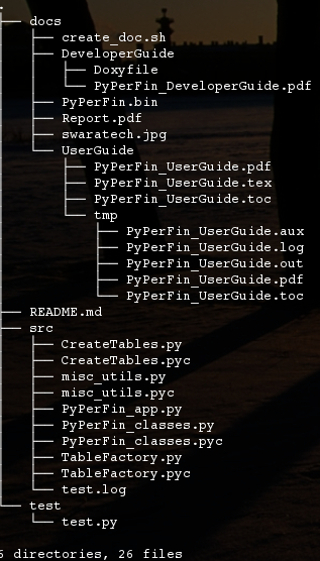
\includegraphics[scale=0.9]{FolderStructure.jpg}
\caption{Folder Structure}
\end{figure}



\chapter{Examples}
\section{To Generate Report}
python PyPerFin.py
\section{To add expense: COMMUTATION for Apr2013}
python PyPerFin.py \--\--o 2 \--\--c 4 \--\--fm Apr2013 \--\--v 2300
\section{To add expense: FUEL for current month}
python PyPerFin.py \--\--o 2 \--\--c 2 \--\--v 1850
\section{To add investment under IND\_EQUITY of type 2}
python PyPerFin.py \--\--o 2 \--\--c 2 \--\--fm Apr2013 \--\--v 9850 \--\--d 30Apr2013 \--\--cm 9MGH8G
\section{To add income under DIVIDEND for current month}
python PyPerFin.py \--\--o 2 \--\--c 2 \--\--v 1850 \--\--d 30Apr2013 \--\--cm 9MGH8G

\end{document}
